%************************************************
\chapter{Analysis and methodology}\label{ch:objectives}
%************************************************

% descripción del proyecto: objetivos, metodología: pasos del diseño y desarrollo, ver figura 3.1 (elección de sensores: computing offloading), contexto (partimos de ABC4T: recordar P2ABCE y que se basa en tarjetas), entorno de desarrollo (meter elección del Omega2, LEDE, teoría de APDUs, código heredado) el sw, los tests p2abce puro, 


%TODO resumir organización del capítulo
% Incluir bibliografía: vanet, wiki


In this chapter we describe the project objectives, and the methodology followed during its development. In section ... TODO

\section{Project description}

The purpose of this project is the integration of IBM's privacy preserving solution, Idemix, in the environment of the Internet of Things. The objective is to design a general solution for the existing IoT devices and systems, without compromising any feature of Idemix, and provide a working PoC in a real IoT environment, even though it isn't the most constrained scenario. The project is aimed to be used in privacy preserving environments, providing security for IoT, controlling what data is being disclosed and to whom. In a smart city project, citizens data can be privatized and continue to offer the benefits of the sensors around. Authorized personnel can disclose the information when required, like firefighters that could access a building sensors to know how many people and what conditions they are in, in case of a emergency; and keep such invasive data private to other non-critical services, for example, only giving a proof that there are more than a minimum number of people in the building, to activate or deactivate the air-conditioning system.

\hfil

We will divide the project in various \textbf{objectives}, starting from the principal goal, dividing our work in different categories.

\hfil

\paragraph{Idemix and the IoT}
We part from this main objective, integrating IBM's privacy preserving system in the IoT environment. 

\paragraph{Analysis} Study the state of the art for Idemix and the IoT, analyzing related projects like ABC4Trust's \ac{P2ABCE}, papers with similar approaches, and our task is to consider the best fitting solutions from where to start.

\paragraph{Design and implementation} After studying the existing works, we must give a formal solution to be implemented. This includes the theoretical architecture, the steps to take, the software to implement, the hardware to use, and any simplifications to leave as future work.

Our \textbf{software} objectives include making it easily maintainable, structured and extensible, from the IoT and original project perspectives, that is, the IoT solution must be interoperable with other non-IoT solutions, now and in the future, with minimal effort, given new IoT systems or changes in the cryptographic protocols.

Our \textbf{hardware} objective is to use devices as constrained as possible. But considering our early situation in the project, we will use IoT devices that ease testing and development, having in mind the other devices, and what specific steps we should take for them in the future.

\paragraph{Validity and evaluation} Deploy a \ac{PoC} in a \textbf{real scenario}, without the need of simulators, checking it works as expected, and measuring its performance.



\section{Methodology}

Giving the vast range of IoT devices, a one-for-all solution must take in consideration multiple requirements and limitations. We will break down the original system, Idemix and P2ABCE, analyze every part of it and categorize them. We will consider what components are mandatory to be executed in the target device and which ones the devices would be able to execute.

Devices with equivalent processing power to smart phones are capable to execute the current Java implementations of P2ABCE and Idemix, but the most constrained ones can't handle the entire system, only the key cryptographic operations.

Using the technique known as \textit{Computation Offloading} we will design an IoT architecture where the most constrained targets can keep their private keys and certificates secure in the same device, and act as any other User in the P2ABCE system. Studying the P2ABCE architecture and implementations we will identify those mandatory operations to be executed in the constrained device, and how to communicate efficiently during the delegation.

After the technical design, we will implement the PoC, using software designs patterns known to many professionals, that will improve the maintainability of the project, for improvements and fixes. Taking advantage of this practices, we can document the immediate steps for future developers, how to reimplement certain interfaces when porting the application to a new system, or where the core logic lies for future protocol changes.

Finally, the PoC must be evaluated to assert we achieved our goals, and measure its performance, judging if it could be fitting for real IoT environments.



\section{Analysis of P2ABCE}

A Privacy Preserving Attribute Based Credential system is composed by several actors, each one of them with different roles. One entity could act with more than one role, e.g., an Issuer could also act as a Verifier, but one can assume each actor acts with one role at a time.


The roles are:


\begin{figure}[bth]
	\begin{center}
		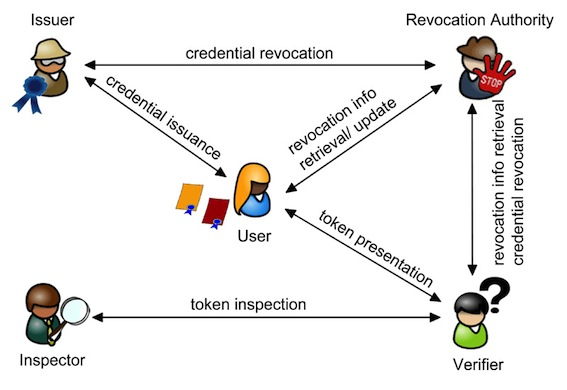
\includegraphics[width=\linewidth]{gfx/actors}
	\end{center}
	\caption{Entities in a P2ABC System}
	\label{fig:actors}
\end{figure}

\begin{itemize}
	\item \textbf{Issuer}\\
	In the ABC infrastructure, the Issuer is a trusted entity responsible for issuing credentials, vouching for the correctness of the information contained. Each Issuer generates a secret key and publishes the Issuer parameters that include the corresponding public verification key.
	
	\item \textbf{User}\\
	Entities that collect credentials from various Issuers. They can decide between all their credentials which attributes and values to present when making assertions about their identity to service providers.
	
	\item \textbf{Verifier}\\
	A service provider that protects access to a resource by imposing restrictions on the credentials that users must own and the information from these credentials that users must present in order to access the service.
	
	\item \textbf{Revocation Authority} (optional)\\
	This entity is responsible for revoking issued credential, preventing their further usage to generate a presentation token. Each revocation authority generates and publishes its revocation parameters.
	
	\item \textbf{Inspector} (optional)\\
	The Inspector's duty is to de-anonymize the user's presentation token under specific circumstances (e.g. misuse or liability). At setup, each inspector generates a private decryption key and a corresponding public encryption key. Usually, the capability of inspection should be bonded to privacy protection laws.
	
\end{itemize}

To sum up, an attribute-based credential contains attribute-value pairs that are certified by a trusted Issuer. A credential can also specify one or more Revocation Authorities who are able to revoke the credential if necessary. Using her credentials, a User can form a presentation token that contains a subset of the certified attributes, provided that the corresponding credentials have not been revoked. Additionally, some of the attributes can be encoded in the presentation token so that they can only be retrieved by an Inspector. Receiving a presentation token from a User, a Verifier checks whether the presentation token is valid w.r.t. the relevant Issuers and Inspector's public keys and the latest revocation information. If the verification succeeds, the Verifier will be convinced that the attributes contained in the presentation token are vouched by the corresponding Issuers.


\hfil

In the P2ABCE repository \citep{p2abcurl} there is available the project's code, divided in two solutions: a complete P2ABCE implementation in Java and a MULTOS smart card implementation as PoC for the project.

\subsection{P2ABCE Code Structure and REST Services}

The Java code is managed by a Maven project, structured using various known design patterns, but not of our interest. The part we are actually interested in are the \textit{REST Services} and their use of the \textit{Components} classes, where the smart card's logic and use are defined.

P2ABCE project is based on the concept of smart cards, virtual or physical, to store the credentials. An interface is defined to communicate with these smart cards, and then different implementations allow to use either \textit{Software Smartcards} or \textit{Hardware Smartcards}. 

The \textit{SoftwareSmartcard} class implements the interface in Java, suitable for applications using P2ABCE self-storing digital smart cards, like a virtual wallet.

The \textit{HardwareSmartcard} class uses the standard APDU messages (\ref{subsec:APDU}) to interact with smartcards. P2ABCE defines the necessary APDU instructions for the smart card needed to implement each method of the interface. It relies on \textit{javax.smartcardio} abstract classes (implemented by Oracle in their JRE) to communicate the smart card reader and the smart card. This way, it doesn't matter what manufacturer issues the smartcard, or if it's an Android device with NFC, if they support the APDU instructions, P2ABCE will work with them.

\begin{figure}[bth]
	\begin{center}
		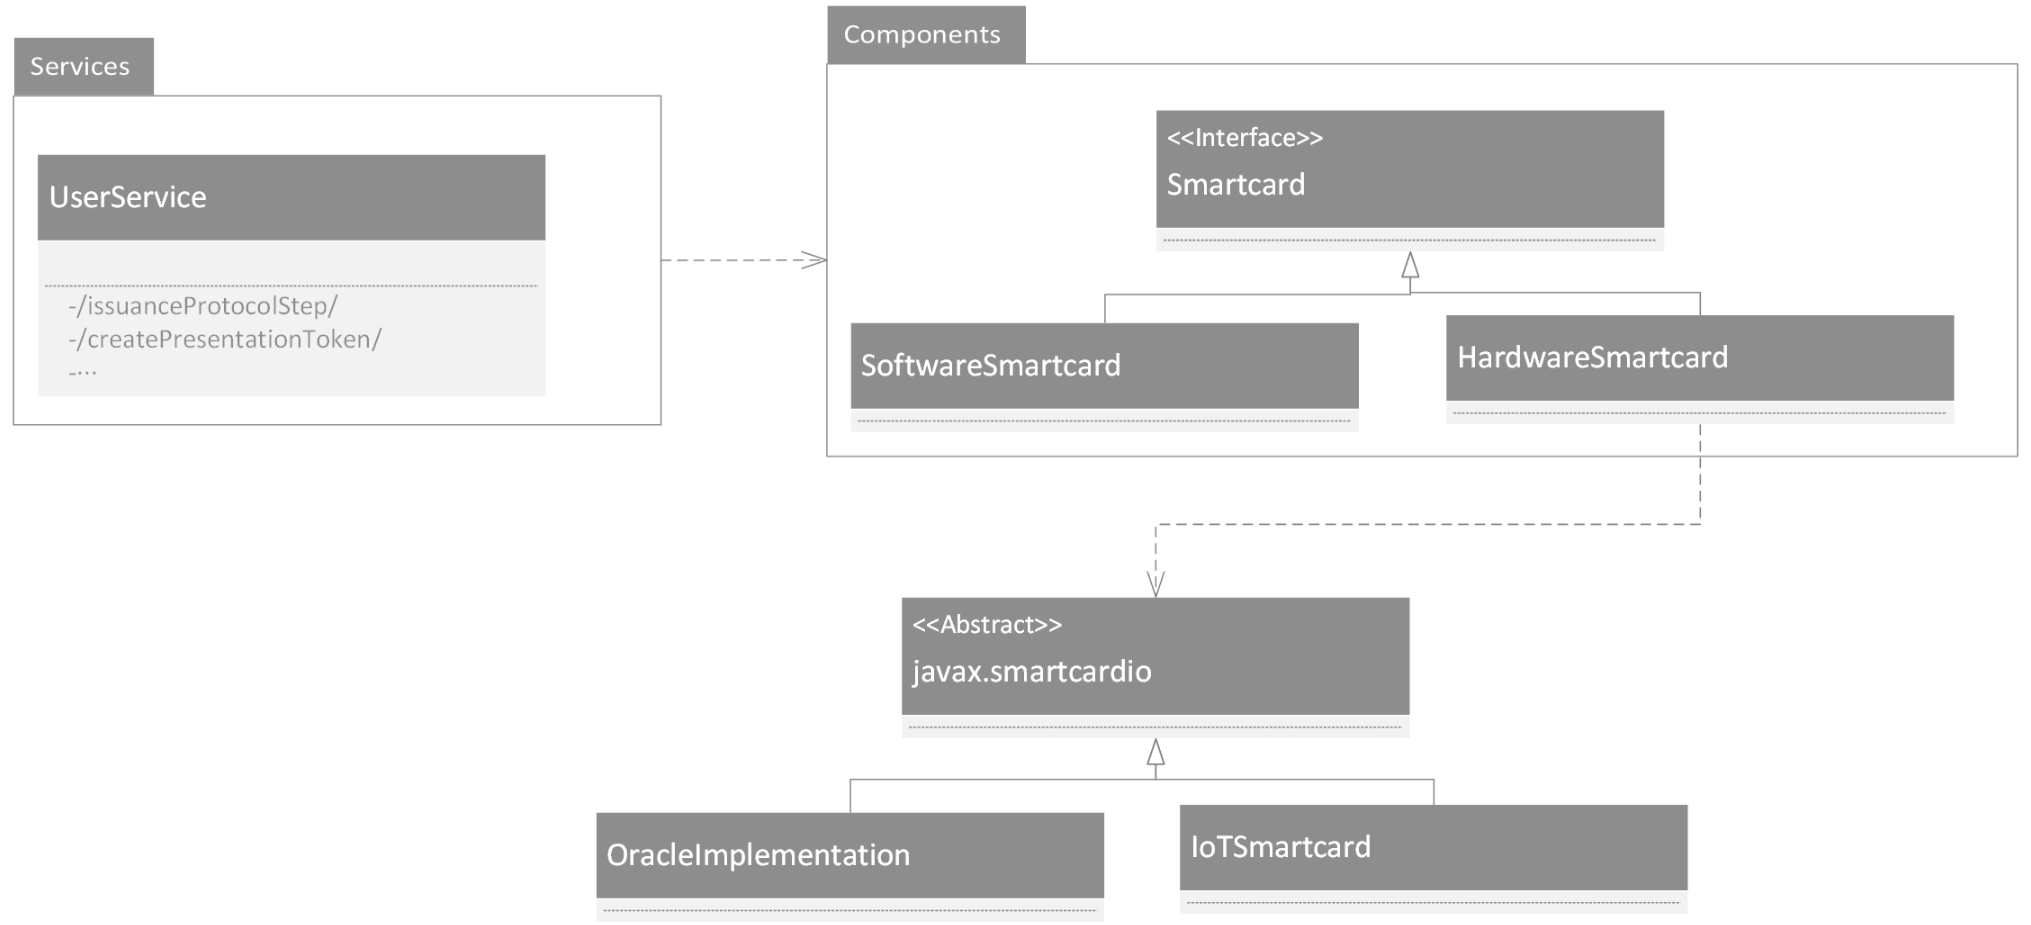
\includegraphics[width=\linewidth]{gfx/p2abceBasicUML}
	\end{center}
	\caption{Basic P2ABCE structure}
	\label{fig:p2abceBasicUML}
\end{figure}


\hfil

The project also provides a set of REST services to control each role of the P2ABCE systeam (User, Issuer, Verifier, Inspector, etc.). The methods implemented include the creation of \textit{Software} smart cards within the User Service, and store them in a data base for future REST calls that may need them.

The services receive parameters like the length of the cryptographic keys, IDs, or XML files to parse. The REST API is not meant for a User Service to communicate with an Issuer Service, for example, but for the User actor to call the Engine through the User Service, to perform specific actions, and then the Service returns the response XML. Those XML files are the way to communicate two different actors. The transmission method to exchange the XML depends on the specific scenario.



\subsection{ABC4Trust Card Lite}

As a PoC the P2ABCE project includes a smart card reference implementation, the ABC4Trust Card Lite \citep{ABC4TCardLite}. It supports device-bound U-Prove and Idemix, and virtually any discrete logarithm based pABC system.

Version 1.2 is written for \texttt{ML3-36K-R1} MULTOS smart cards, with approximately 64KB of EEPROM (non-volatile memory), 1KB of RAM and an Infineon SLE 78 microcontroller, a 16-bit based CPU aimed for chip cards.

The card stores the user's private key $x$ and any \ac{BLOB} that the P2ABCE may need (like user's credentials). Then P2ABCE delegates the cryptographic operations on the smart card, that operates with $x$.

\begin{figure}[bth]
	\begin{center}
		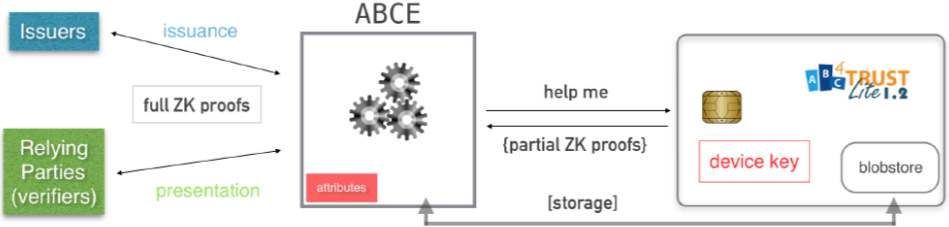
\includegraphics[width=\linewidth]{gfx/ABC4TCardLite}
	\end{center}
	\caption{ABC4Trust Card Lite}
	\label{fig:ABC4TCardLite}
\end{figure}

The cryptographic operations performed by the smartcard are the modular exponentiation and addition used by ZKPs based on the discrete logarithm problem.

\hfil

The code is available from the P2ABCE's repository and has some good and bad points to have in count:

The best asset of this code is that it's written in C aiming to a very constrained device, with very limited memory and similar computational power to many other IoT devices.

The code uses some good practices when programming for IoT devices, like using \textit{union} data types for variables that will be stored on the same data location, but at different times, minimizing this way the use of RAM and making code readability better; or like the strong use of pointers and \textit{memcpy} calls to copy structures with multiple variables as arrays of bytes.


Although, among the many drawbacks, we could highlight the \textit{awful} coding style, the strong dependency on MULTOS framework and many bugs found. 

The code is structured in two files, \textit{main.h} and \textit{main.c}, with around $550$ and $5200$ lines of code, respectively.

The file \textit{main.h} is mostly a reimplementation in assembly MEL code of some MULTOS functionality already offered by their API.

The \textit{main.c} consists on nearly $600$ lines of variables and data structures declarations; followed by the \textit{main()} function, a $2600$ lines long \textit{switch-case} expression, with practically no comments; and to conclude, the implementation of thirty functions called \textit{Subroutines} at the end of the file, around other $2000$ lines of code.

\hfil

At this stage, we have two options to implement our IoT device compatible with P2ABCE:

\begin{itemize}
	\item Implement in C the \textit{Smartcard} interface used by P2ABCE architecture, and use some communication protocol to remotelly call the methods from the machine running the P2ABC Engine.
	\item Present the IoT device as a hardware smart card, using the APDU protocol (already defined, standard and with minimal overload). Providing a \textit{javax.smartcardio} ``IoT implementation'' to communicate with the IoT device through a transmission protocol, making the already existing \textit{HardwareSmartcard} class compatible with the new \textit{IoTSmartcard} running in the IoT device.
\end{itemize}

Even with the problematic to maintain or even understand the code of ABC4Trust Card Lite, once one studies MULTOS framework in deep and applies many refactoring techniques to the code, it becomes the best starting point for the IoT version, making us opt for the second option.





\section{Preliminaries about smart cards}

In this section we will introduce a brief description of the APDU standard protocol, and the MULTOS framework used by the ABC4Trust Card Lite.


\subsection{Smart Card Communication Protocol}\label{subsec:APDU}

To communicate the smart cards and the reader the ISO/IEC 7816-4 \citep{APDUISO} specifies a standardized protocol .

The messages, also kown as \acp{APDU}, are divided in APDU Commands and APDU Responses.

\textbf{APDU Commands} consist in 4 mandatory bytes (CLA, INS, P1, P2), and an optional payload.

\begin{itemize}
	\item CLA byte: Instruction class. Denotes if the command is interindustry standard or proprietary.
	\item INS byte: Instruction code. Indicates the specific command.
	\item P1, P2 bytes: Instruction parameters.
	\item Lc, 0-3 bytes: Command data length.
	\item Command data: Lc bytes of data.
	\item Le, 0-3 bytes: Expected response data length.
\end{itemize}

This way, minimal number of bytes are needed to transmit commands to the smart card, allowing manufacturer's personalization of the smart card behavior and capabilities along with standard operations.

\begin{figure}[bth]
	\begin{center}
		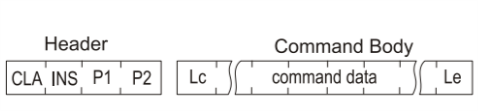
\includegraphics[width=0.55\linewidth]{gfx/APDUCommand}
	\end{center}
	\caption{APDU Command}
	\label{fig:APDUCommand}
\end{figure}


\textbf{APDU Responses} are generated inside the smart card, always as an answer to an APDU Command. They consist on an optional payload and two mandatory status bytes.


\begin{itemize}
	\item Response data: At most Le bytes of data.
	\item SW1-SW2 bytes: Status bytes. Encode the exit status of the instruction.
\end{itemize}

\begin{figure}[bth]
	\begin{center}
		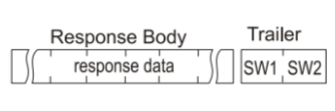
\includegraphics[width=0.55\linewidth]{gfx/APDUResponse}
	\end{center}
	\caption{APDU Response}
	\label{fig:APDUResponse}
\end{figure}




\hfil


The transmission protocol varies between different types of readers and smart cards (e.g. chip, contact-less), but what is common between every smart card interaction, is the \textit{APDU Command-Response Dialogue}. As long as the smart card has a power supply, it can maintain the memory in RAM between APDU Commands, what allows to do in two or more steps complex operations, transmit more bytes than a single APDU can admit, etc.

\hfil




\begin{figure}[bth]
	\begin{center}
		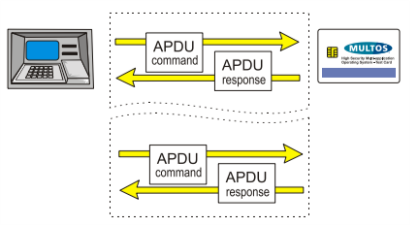
\includegraphics[width=0.75\linewidth]{gfx/APDUdialog}
	\end{center}
	\caption{APDU Command-Response Dialogue}
	\label{fig:APDUdialog}
\end{figure}

Originally, the Lc and Le bytes had only 1 byte, if present, restricting the payload data to be at most 256 bytes long. An extension to the protocol changed the meaning of a Lc or Le 0x00 byte (256 bytes long payload), so when the byte corresponding to Lc or Le started with 0x00, the next two bytes where the real length.  With this, an Extended APDU lets up to $65536$ bytes of data.

The problem here, is that not all readers or smart cards support extended APDUs. Originally, to send more than 256 bytes of data in an APDU Command, a \textit{Put Data} instruction is defined, so the smart card stores the payload in a buffer, until other APDU Command indicates how to use it.

To send more data in an APDU Response, the status bytes are set to: SW1=0x61 and SW2 to the remaining bytes to send. Because a smart card can't send APDU Commands, the card terminal must send a \textit{GET RESPONSE}, a special APDU Command, with Le set to the number of bytes specified in SW2. Iterating this process, the smart card can send as many bytes as it wants as Response.

With the introduction of Extended APDUs, this technique is no longer needed.






\subsection{MULTOS}

MULTOS is a multi-application smart card operative system, which provides a custom developing environment, with rich documentation \citep{MultosTechLib}. MULTOS smart cards communicate like any other smart card following the standard, but internally offers a very specific architecture, affecting the way one must code applications for it.

In this section we will present the main characteristics of a MULTOS smart card that shaped the ABC4Trust Card Lite code and that we had to be aware of when adapting it to IoT devices.

\paragraph{MULTOS programming languages} A native assembly language called MEL, C and, to a lesser extent, Java, are the available languages to code for MULTOS. In our case, ABC4T Card Lite uses MEL and C.

\paragraph{MULTOS Workflow}

Most of the transmission and communication process is done by MULTOS core, and it then selects, based on the CLA byte of the APDU, the application to load. This application is what most developers will only worry about, and is where their $main()$ function will start.

\begin{figure}[bth]
	\begin{center}
		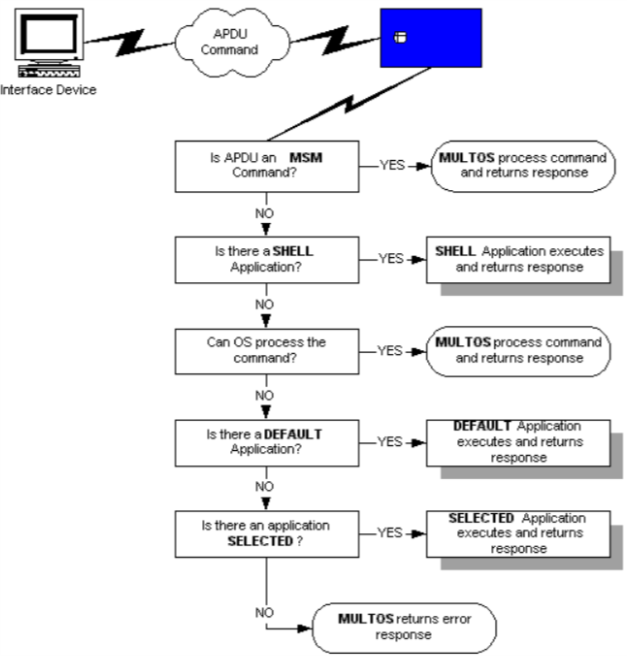
\includegraphics[width=0.6\linewidth]{gfx/multosWorkflow}
	\end{center}
	\caption{MULTOS Workflow}
	\label{fig:multosWorkflow}
\end{figure}

The application uses then the \textit{multos.h} file that declares multiple global variables already loaded with the needed data, including the APDU Command bytes.

Now the developer is in charge of checking what instruction was sent and if the APDU has the expected ISO Case. If everything is ok, code what needs to be run and write in specific data space the APDU Response bytes, call \textit{multosExit()} and MULTOS will be in charge to send the APDU Response.

In summary, our application starts with all data loaded and exits without worrying how to send the answer. A very comfortable workflow that we must now implement for our IoT device if we would want ABC4T Card Lite code to work.

\paragraph{MULTOS Memory Layout}

Each application in MULTOS has access to a specific memory layout, divided in different categories:

\begin{figure}[bth]
	\begin{center}
		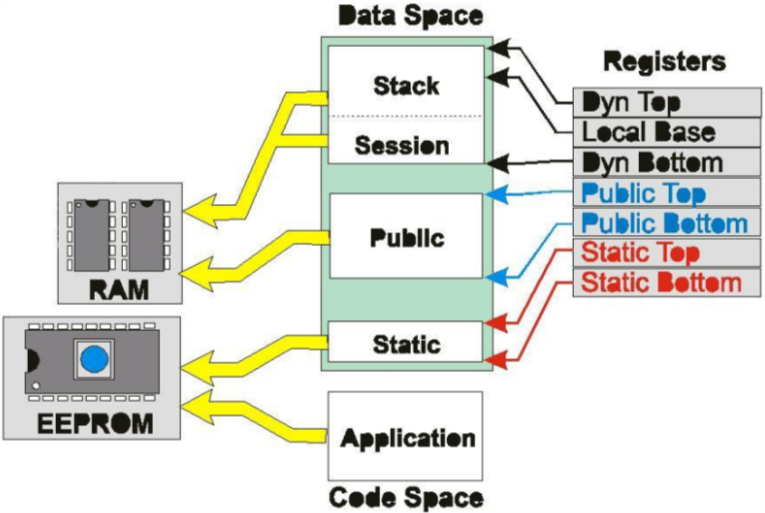
\includegraphics[width=0.8\linewidth]{gfx/multosMemLay}
	\end{center}
	\caption{MULTOS Memory Layout}
	\label{fig:multosMemLay}
\end{figure}


The Code Space is where the application code is stored.
The Data Space is divided in Static memory, Public memory and Dynamic memory.

\textbf{Static memory} are the application variables declared after the specific \textit{\#pragma melstatic} compiler directive. These variables are stored in the non-volatile EEPROM, and any write is assured to be saved because they are not loaded into RAM.

\textbf{Public memory} can be seen as the input/output buffer for applications and MULTOS system. The APDU header appears at the top of Public, and command data at the bottom. The application writes then the APDU Response bytes in Public, at specific position (see \autoref{fig:multosPubMem}). To declare variables in this data space, the \textit{\#pragma melpublic} directive is available.

\textbf{Dynamic memory} works like usual program memory, with Session Data storing global variables and the Stack. The limited size of RAM in IoT devices and smart cards makes the use of dynamic memory not advisable. The compiler directive to use Session Data is \textit{\#pragma melsession}.


\begin{figure}[bth]
	\begin{center}
		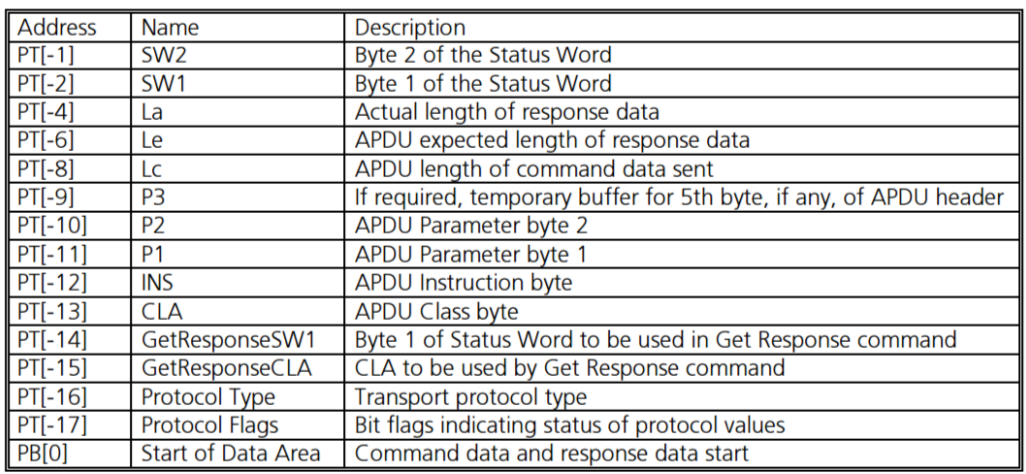
\includegraphics[width=\linewidth]{gfx/multosPubMem}
	\end{center}
	\caption{MULTOS Public Memory Data Map}
	\label{fig:multosPubMem}
\end{figure}


\hfil


With regards to primitive types, to avoid confusion with their sizes, MULTOS defines and uses the following data types specified in \autoref{fig:multosDataTypes}. It's important to notice that MULTOS is Big Endian
\marginpar{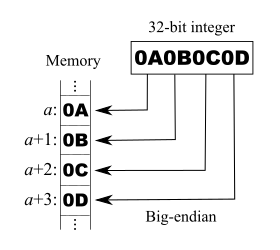
\includegraphics[width=\linewidth]{gfx/Big-Endian}\\Big-Endian, Wikipedia}
and when storing structures there is no padding between defined variables, unlike modern compilers that perform data structure alignment \citep{dataStructAlign} for performance.

\begin{figure}[bth]
	\begin{center}
		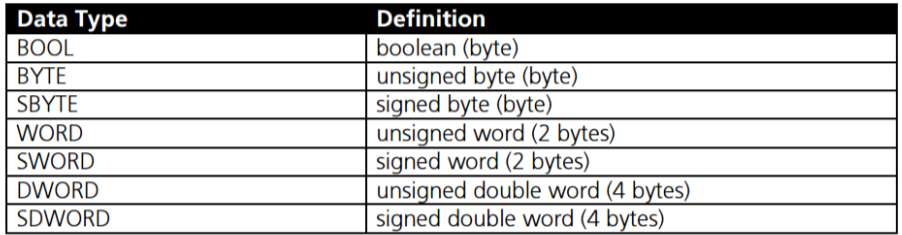
\includegraphics[width=\linewidth]{gfx/multosDataTypes}
	\end{center}
	\caption{MULTOS Data Types}
	\label{fig:multosDataTypes}
\end{figure}


\paragraph{MULTOS Standard C-API}

A collection of more than a hundred functions are provided for arithmetic, cryptography, memory and smart card operations. The \textit{multos.h} interface provides access to these functions, that ultimately call their respective primitive instructions in assembly code. The primitive instructions are but a system call with an operation code, loading data in the needed registers. Therefore,  no implementation for these tools is available, nor in C, nor in assembly code.

Nevertheless, the C-API documentation \citep{MultosTechLib} provides rich description for each function.




\hfil

\section{Development environment}


For almost every IoT device in the market, there exists a C compiler and many frameworks available to build firmware binaries, like Arduino Core, Contiki, Mongoose OS, ThreadX OS, OpenWrt, LEDE, proprietary SDKs, etc. Each firmware targets a specific range of devices, depending on processing power and memory limitations. For example, Arduino and Contiki aim for very constrained microcontrollers, like Atmel's ATmega or TI's MSP430, but can also be used in ESP8266, a more powerful device, with WiFi capabilities.
\marginpar{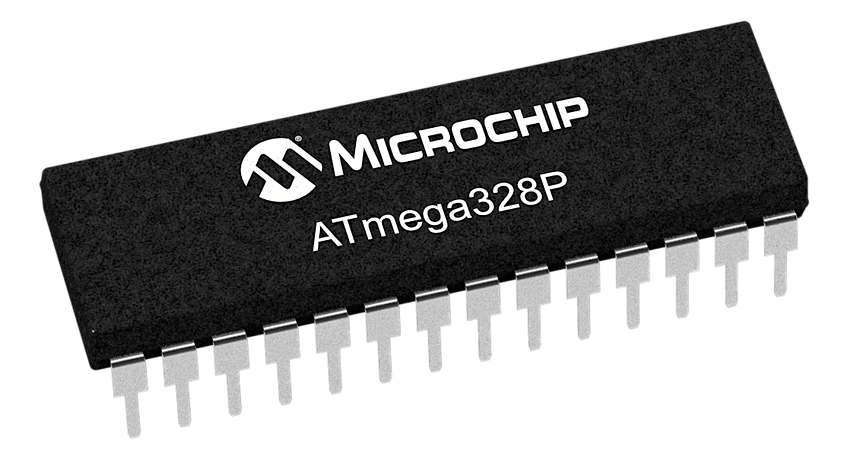
\includegraphics[width=0.8\linewidth]{gfx/ATmega328P}\\$ATmega328P$}

Starting a big project development for \ac{IoT}, aiming the most constrained devices may not be a good idea. The lack of usual OS tools, like POSIX, threads, or minimum I/O, like a terminal, can make debugging a tedious task. With good programming practices, one can start from the top and slowly end with more constrained devices and reliable code.


For this reason, the current \ac{PoC} is developed on LEDE, Linux Embedded Development Environment \citep{ledeproject}, using the Onion Omega2 development board. Although the Omega2 uses LEDE, its microcontroller is also listed as compatible with ThreadX OS \citep{THREADX}, a Real-Time Operative System for embedded devices, therefore, the performance measured in our PoC can be relevant to real scenarios with similar hardware.

The PoC will take advantage of the Linux system using mainly files and sockets like in any other Linux desktop distribution, so we can focus on the project itself rather than the specific platform APIs for storage and connectivity.


\hfil

The project development is divided between the IoT device code and the P2ABCE services. To ease the setup of new developing machines, we will use Docker to deploy containers ready to compile the code.

\hfil

P2ABCE is already written in Java and uses Maven to manage dependencies. The project needs some minor changes to work with our IoT architecture. Any text editor or Java IDE is suitable for the development, because the compilation is done through the terminal, with Maven commands.

We compile the project inside a Docker container, with OpenJDK 7, Maven 3 and Idemix 3.0.36, following the project \href{https://github.com/p2abcengine/p2abcengine/wiki/How-to-Build-the-ABC-Engine}{instructions} to use Idemix as the Engine for P2ABCE.

\hfil

We can assume all IoT devices have a C cross-compiler, some even a C++ cross-compiler. The worst case scenario is that one must write assembly code, and that code will be specific of that target, so we won't consider them.
If now we focus on the most constrained devices, we could find out that for some we can't use C++, some may not have many usual libraries, moreover, the memory limitations they face make practically impossible to use dynamic memory, if we want to avoid many execution malfunctions.

For that reason, the developed code for IoT devices should be written with standard C, without using dynamic memory or third party libraries.

\hfil


To manage the PoC code we chose CMake, providing many advantages over Makefiles:

\begin{itemize}
	\item Cross-platform. It works in many systems, and more specifically, in Linux it generates Makefiles.
	\item Simpler syntax. Adding a library, files to compile, set definitions, etc. can be done with one CMake command, with rich documentation on the project's \href{https://cmake.org/cmake/help/latest/}{website}.
	\item Cross-compilation. With only a \href{http://www.vtk.org/Wiki/CMake_Cross_Compiling#The_toolchain_file}{\small{CMAKE TOOLCHAIN}} file, CMake sets up automatically the cross-compilation with Makefiles and the C/C++ cross-compiler provided.
\end{itemize}


\hfil

Although the ideal final code is written in pure C, without external libraries or dynamic memory, the PoC uses three major libraries:

\begin{itemize}
	\item OpenSSL: Provides reliable and tested AES128, SHA256 and random number generator implementations.
	\item LibGMP: Provides multiprecision integer modular arithmetic.
	\item cJSON: Provides a JSON parser to store and read the status of the device, in a human readable way.
\end{itemize}

These three libraries are used to implement different interfaces in the project, and C implementations of these interfaces should replace the external libraries in the future.

\hfil

Finally, we use Docker to deploy the compilation environment. Our container includes CMake and the LEDE SDK \citep{ledeproject}, configured for the Omega2 target, the device chose for the PoC.

The Dockerfiles and CMake cross-compilation toolchain can be found in \autoref{ch:docker}.
